
\documentclass{leaflet}
\usepackage[ngerman]{babel}
\usepackage[utf8]{inputenc}
\usepackage{blindtext}
\usepackage{biolinum}
\renewcommand\rmdefault{\sfdefault}% Verwende serifenlose Schrift
\usepackage{mwe}% Dummy Bilder
\usepackage{xcolor}
\AddToBackground{1}{\put(0,0){\textcolor{green!20}{\rule{\paperwidth}{\paperheight}}}}% Farbiger Hintergrund für 1. Seite


\begin{document}
\title{Leerstand-kreativ-nutzen-Projekt in der Havellandstraße 20 (Eberswalde - BV)}
\author{Hebewerk e.V.}
\date{März 2015}
\maketitle
\thispagestyle{empty}% Keine Seitenzahlen
\clearpage

\section{Diese Räume sind, was ihr draus macht} 
Hier stehen euch freie Räume zur kostenlosen, gemeinschaftlichen Nutzung zur Verfügung. Ihr habt die Möglichkeit, diese Räume nach Absprache zu nutzen. Dafür stehen mehrere Schlüssel zur Verfügung. Schreibt uns dafür einfach eine Mail … , ruft uns an … oder kommt zum nächsten Treffen: 3. 2.,  17.2. (im Schöpfwerk), 3.3., 17.3., 31.3. (in der Havellandstraße)
Hier gibt es die Möglichkeit zum Zeichnen mit freier Software, Elektronik, Raspberry, Chill-out-Abende, Vortrags- und Diskussions-Abende, Gruppen- oder Seminartreffen, Zusammenarbeit mit Geflüchteten … und allem, worauf ihr noch Lust habt! Außerdem ist die Internetnutzung hier möglich.\\
\\ \
\\ \
Wir verstehen uns als parteiunabhängig und antirassistisch. 
\\ \


\clearpage


\section{Projekte}

\begin{description}
\item[CNC-Fräse] Die CNC-Technik ermöglicht das 3D-Fräsen, mit dem kompliziertere 3D-Konturen erzeugt werden können. 

\item[3D-Drucker] Ein 3D-Drucker ist eine Maschine, die dreidimensionale Werkstücke schichtweise aufbaut. Der Aufbau erfolgt computergesteuert aus einem oder mehreren flüssigen oder festen Werkstoffen nach vorgegebenen Maßen und Formen. Beim Aufbau finden physikalische oder chemische Härtungs- oder Schmelzprozesse statt. Typische Werkstoffe für das 3D-Drucken sind Kunststoffe, Kunstharze, Keramiken und Metalle.

\item[Repair-Caf\'{e}] Das Repair Caf\'{e} ist eine gemeinschaftlich organisierte Hilfe zur Selbsthilfe. Getragen wird die Veranstaltung von ehrenamtlich engagierten Helfern und Reparatur-Experten, die ihr Wissen und Können freiwillig und unentgeltlich zur Verfügung stellen. Besucher des Repair Caf\'{e} bringen ihre kaputten oder funktionsuntüchtigen Gegenstände von Zuhause mit. Toaster, Lampen, Föhne… alles, was nicht mehr funktioniert, kaputt oder beschädigt ist, kann mitgebracht werden. Und die Wahrscheinlichkeit ist groß, dass die Reparatur gelingt!


\newpage	

\section{Die beteiligten Initiativen}

\item[Wandelbar] WandelBar ist eine Initiative, die sich vor dem Hintergrund zurückgehender natürlicher Ressourcen, Klimawandel und Krisen aller Art sich mit dem zu beschäftigen, was jede\_r vor Ort selbst tun kann. Wandelbar will auf gute Beispiele, die schon hier in unserer Region bestehen, aufmerksam machen und Menschen zur Mitarbeit in schon aktiven Projekten motivieren, zur Entwicklung weiterer praktischer Ideen anregen und sich mit anderen vernetzen, die sich auch dafür interessieren.


\item[Hebewerk] Das Hebewerk ist eine offene Werkstatt mit offenem Technologielabor, zu dem u.a. das Schöpfwerk, das Repair Caf, 3D-Drucker und CNC-Fräse, die mobile Soundbox, das Lastenrad  und der LINUX-Node gehören. Hier lautet das Motto: Nicht wegwerfen, verzweifeln oder Trübsal blasen, sondern selber machen!


\item[ALNUS] Die Arbeitsgemeinschaft für Landschaftspflege, Naturschutz, Umweltbildung und Stadtökologie ist ein studentischer Naturschutz-Verein. Unser Name ist Programm: Wir organisieren u.a. den jährlich stattfindenden Eberswalder Frühjahrsputz, die Wiesenmahd, bieten Umweltbildungstage, Vogel- und Fledermausführungen an und im Schulgarten und dem BV-Garten haben Kinder, Studenten und sonstige Interessierte die Möglichkeit, ihr eigenes Gemüse anzubauen.

\end{description}

\clearpage
\section{So erreicht ihr das Haus}
Fahrt mit der Buslinie 861 oder 862 bis zur Haltestelle „Brandenburger Allee“, dann liegt das Haus direkt gegenüber der großen Wiese. Mit dem Fahrrad fahrt ihr am besten über die Rudolf-Breitscheid-Straße ins brandenburg. Viertel und fahrt dann über die Lausitzer Straße und Rathenower Straße zum Haus. 

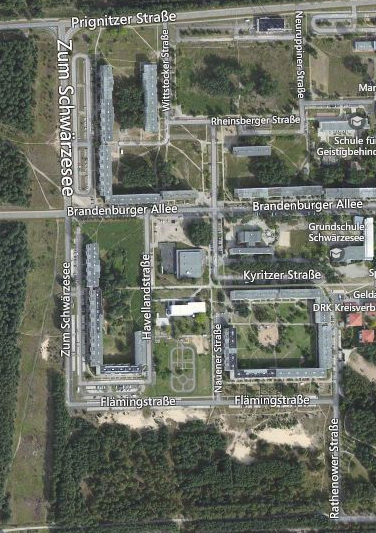
\includegraphics[width=\textwidth]{havellandstrasse}

\section{Termine im März}
\begin{tabular}{llp{5cm}}
3. März	&18h&Hebewerk Jour Fixe\\     
	&19h&Leerstand-kreativ-nutzen Jour Fixe (internes Treffen)\\
	&20h&Leerstand-kreativ-nutzen Jour Fixe (offenes Treffen)\\
\\\
11. März&19h&Chill-out-Abend  - gemütliches Beisammensein\\
\\\
12. März&19h&Wandelbar-Kennenlerntreffen\\
\\\
16. März&19h&ALNUS-Vorstandsversammlung\\
\\\
17. März&18h&Hebewerk Jour Fixe\\
        &19h&Leerstand-kreativ-nutzen Jour Fixe (internes Treffen)\\
	&20h&Leerstand-kreativ-nutzen Jour Fixe (offenes Treffen)\\
\\\
31. März&18h&Hebewerk Jour Fixe\\
	&19h&Leerstand-kreativ-nutzen Jour Fixe (internes Treffen)\\
	&20h&Leerstand-kreativ-nutzen Jour Fixe (offenes Treffen)\\
\end{tabular}	




\end{document}
